Table \ref{tab:allvsall} shows the aggregated metrics for \ac{auroc}, \ac{auprc}, \ac{rmse} and \ac{mae} for distributed, centralised and local models predicting capabilities on each silo. The data refers to the mean of the metric values for all columns tested as targets for all methods and all silos. We also calculated the 95\% confidence interval for each model (local and distributed per silo in order to assess how well the distributed model would work as opposed to the local one per silo. We also calculated the \textit{P} value for the means.
%TC:ignore

\begin{table}[htbp] 
 \setlength{\tabcolsep}{7pt} % Default value: 6pt 
 \renewcommand{\arraystretch}{1.3} % Default value: 1
  \captionsetup{justification=centering} 
\centering
\caption[Metrics for centralised model, distributed model and local model]{Comparison for the centralised model, distributed model and local model (Mean for all model and all columns). Bold for \textit{P} value below 0.05.}
\label{tab:allvsall}
\begin{tabular}{llcccc}
\toprule
 &  & M & SD & 95\% CI & \textit{P}  \\
\midrule
\multirow[t]{3}{*}{AUPRC}
 & distributed & 0.691 & 0.216 & (0.686, 0.696) & - \\
  & centralised & 0.706 & 0.225 & (0.701, 0.711) & \bfseries 1.10e-17 \\
 & local & 0.659 & 0.220 & (0.654, 0.665) & \bfseries 4.71e-05 \\
 \hline

\multirow[t]{3}{*}{AUROC} 
 & distributed & 0.723 & 0.182 & (0.718, 0.727) & - \\
 & centralised & 0.729 & 0.180 & (0.725, 0.734) & \bfseries 2.98e-26 \\
 & local & 0.692 & 0.164 & (0.688, 0.695) & \bfseries 2.48e-02 \\

\hline

\multirow[t]{3}{*}{MAE} 
 & distributed & 2.370 & 1.608 & (2.315, 2.425) & - \\
 & centralised & 2.365 & 1.923 & (2.298, 2.431) & \bfseries 2.23e-04 \\
 & local & 2.527 & 1.799 & (2.465, 2.589) & 9.01e-01 \\

\hline

\multirow[t]{3}{*}{RMSE} 
 & distributed & 21.171 & 46.078 & (19.584, 22.757) & - \\
 & centralised & 19.839 & 28.645 & (18.853, 20.826) & \bfseries 2.92e-02 \\
 & local & 23.771 & 49.776 & (22.057, 25.485) & 1.63e-01 \\
\hline
\end{tabular}
\end{table}





%TC:endignore



%TC:ignore

\begin{figure}[htbp]
\centering
\captionsetup{justification=centering}

\caption{Heatmap of classification algorithm and silo vs Target variable and model type. Value is the \ac{auroc} mean of all 10 experiments. Y axis is the algorithm and silo. X axis is Target variable and Method.}\label{fig:heatmap-cat} 
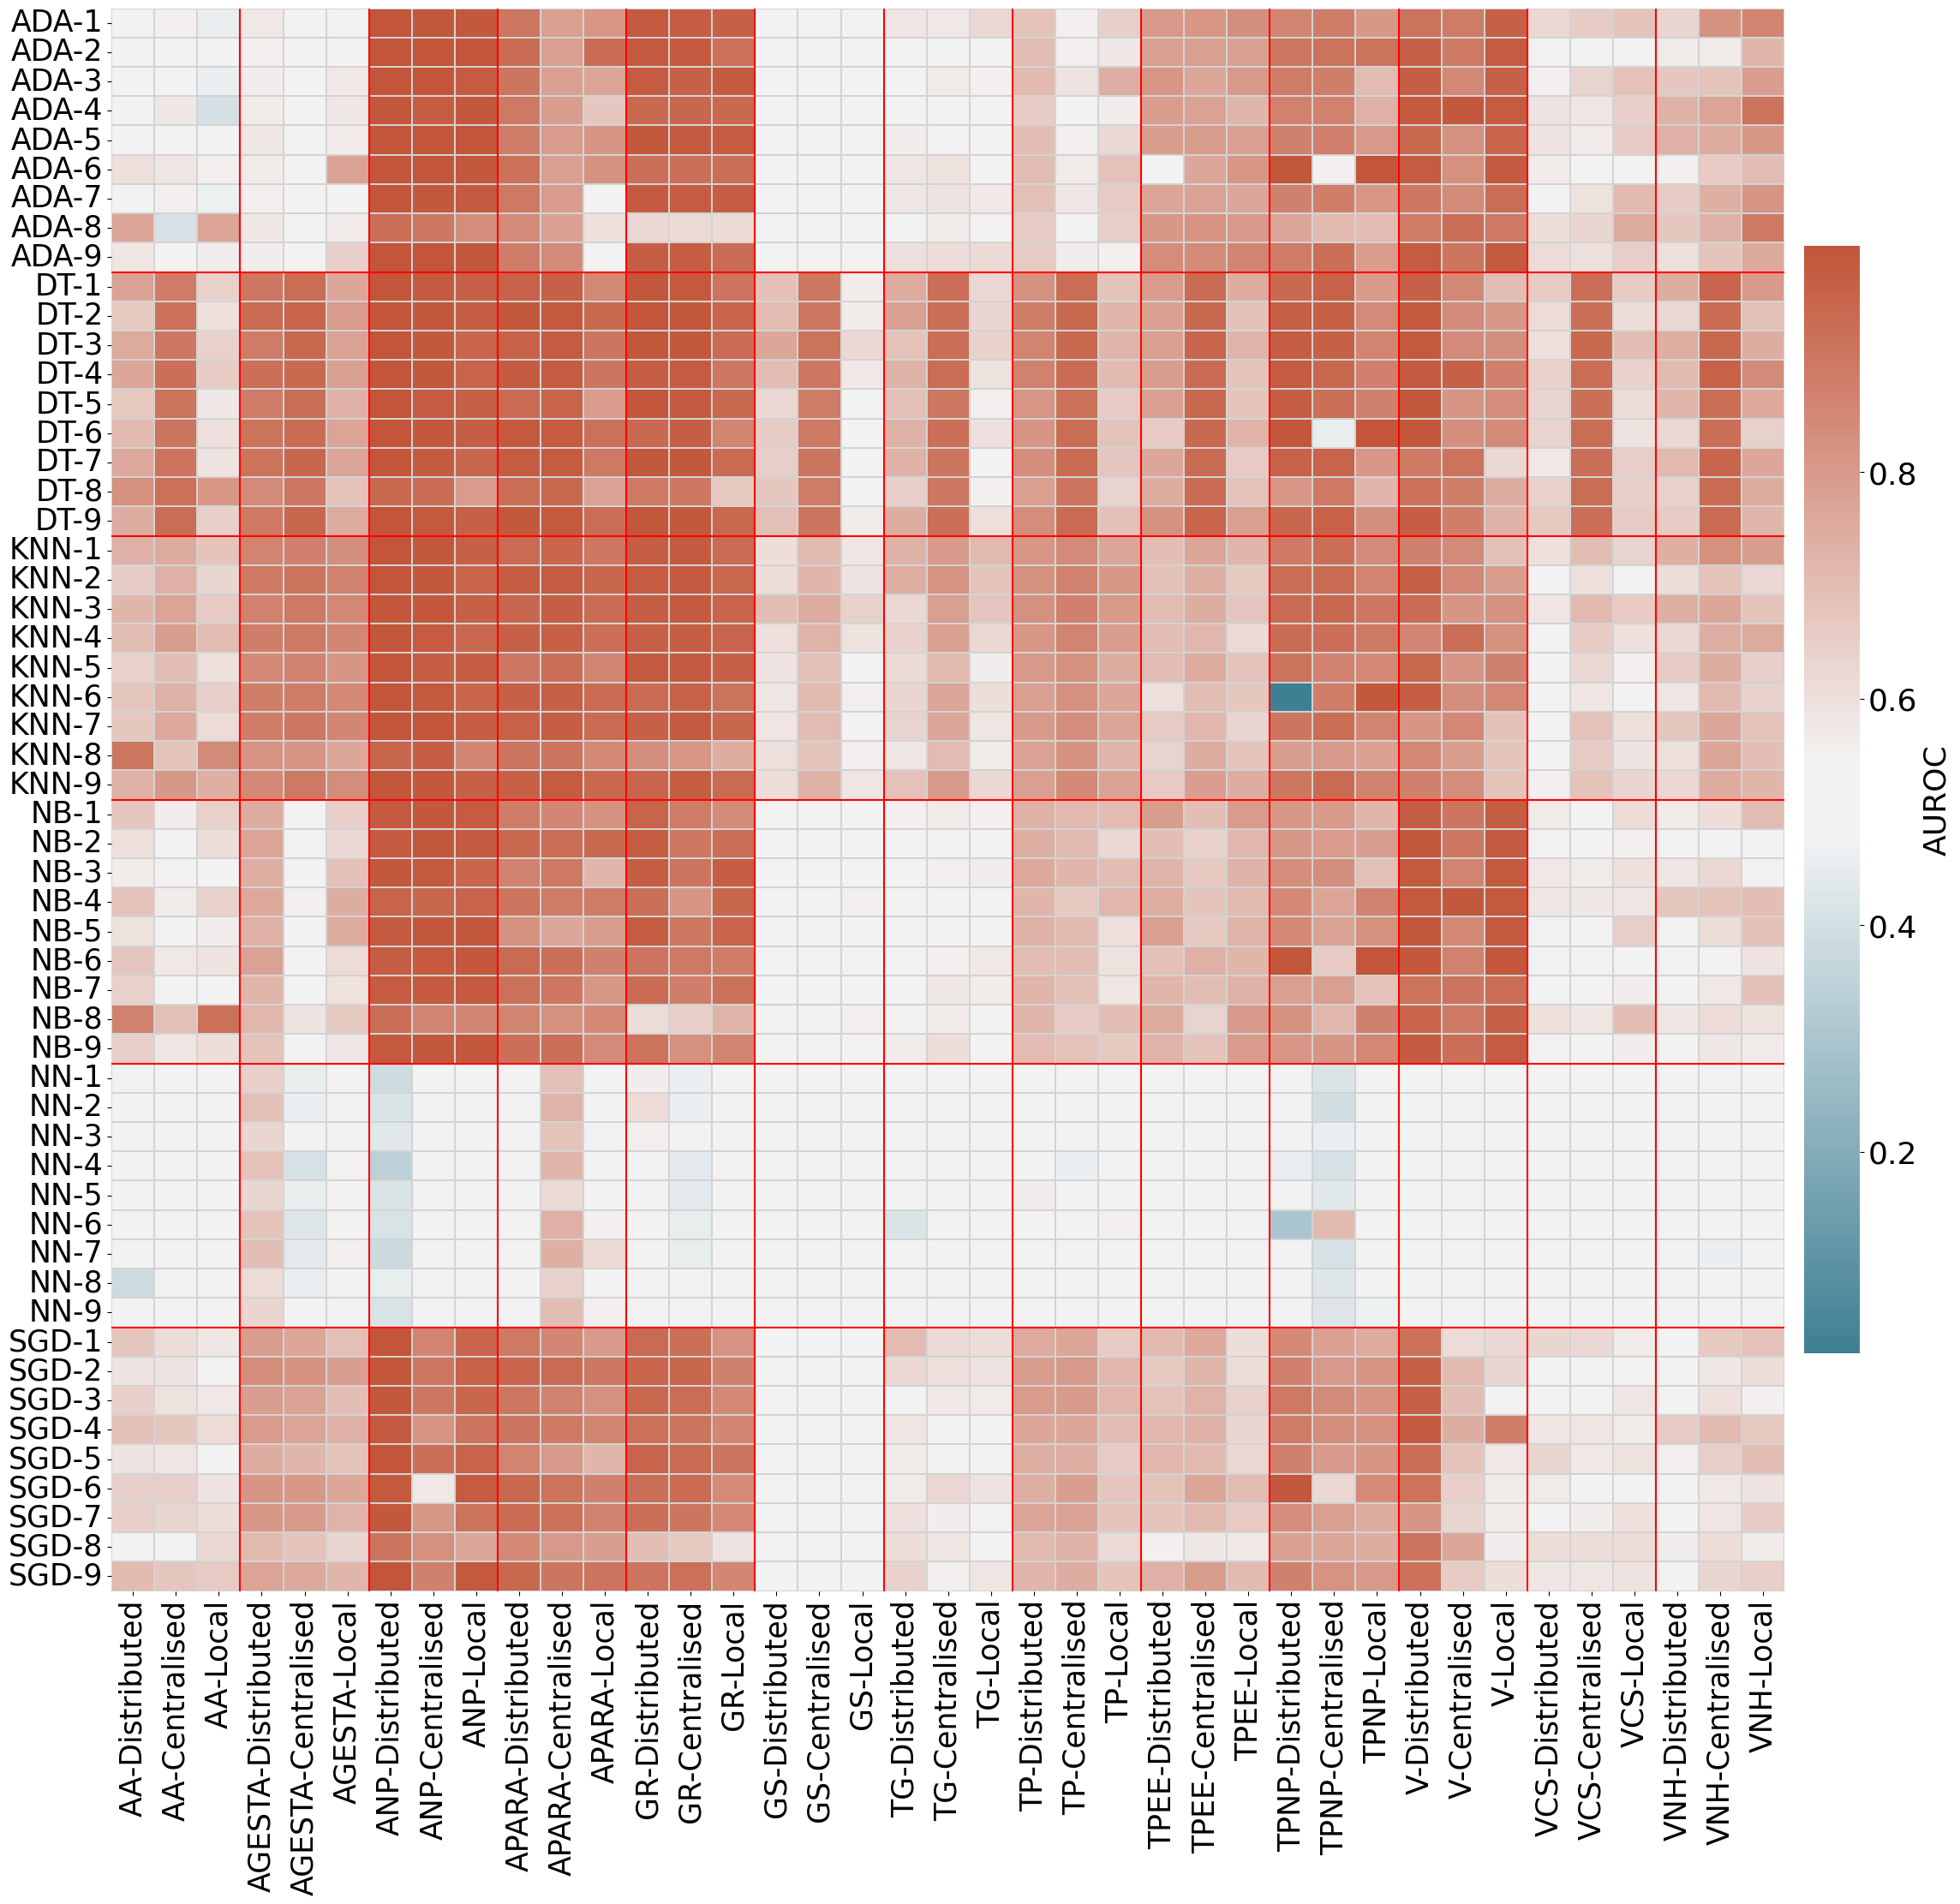
\includegraphics[scale=0.26]{figures/heatmap-class.png}
\end{figure}
%TC:endignore
%TC:ignore

\begin{figure}[htbp]
\centering
\captionsetup{justification=centering}

\caption{Heatmap of regression algorithm and silo vs Target variable and model type. Value is the \ac{mae} mean of all 10 experiments. The y axis is the algorithm and silo. X axis is Target variable and Method.}\label{fig:heatmpa-int} 
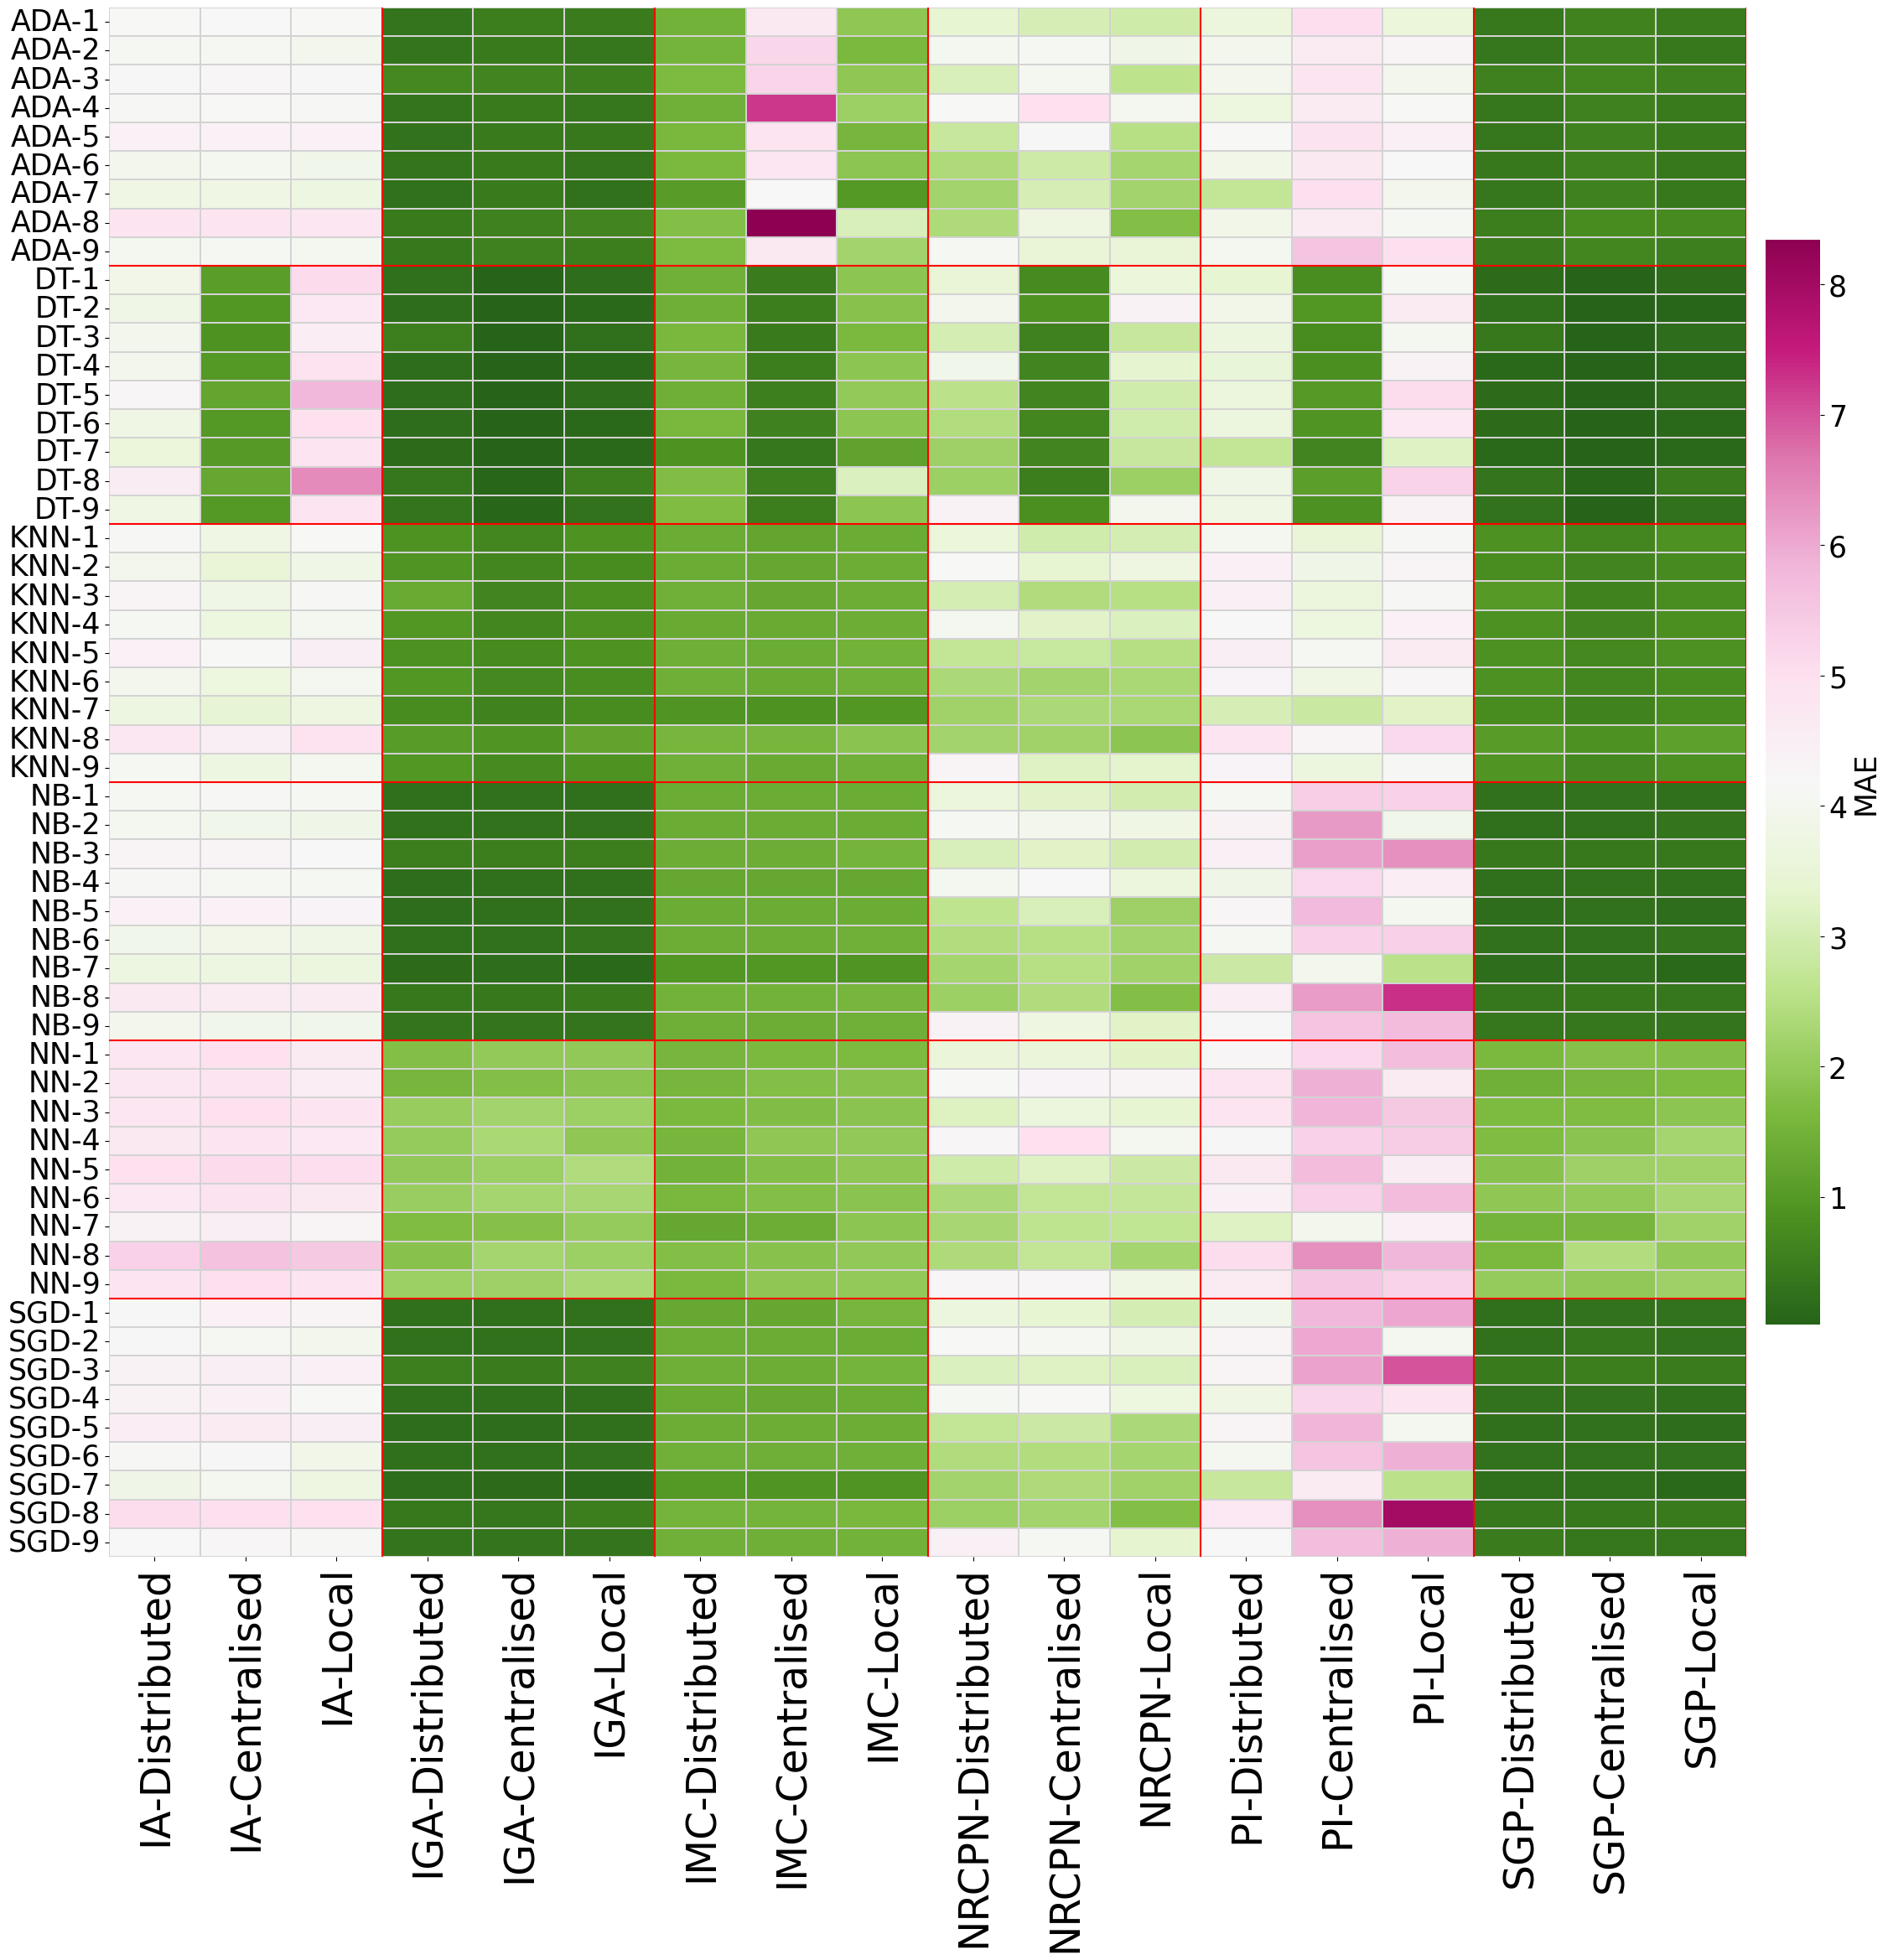
\includegraphics[scale=0.22]{figures/heatmap-reg.png}
\end{figure}
%TC:endignore


\definecolor{Gray}{gray}{0.85} 
 %\newcolumntype{a}{>{\columncolor{Gray}}r} 
 \begin{table}[htbp] 
 \setlength{\tabcolsep}{6pt} % Default value: 6pt 
 \renewcommand{\arraystretch}{1.1} % Default value: 1
  \captionsetup{justification=centering} 
\centering
\caption[Hypothesis testing of Distributed versus Centralised and local models]{Hypothesis testing of Distributed versus Centralised and local for every test. Each cell is the total of distributed model when compared with centralised model (row) and local model (column). ($>$ for better, = for non significance and $<$ for worse)}
\label{tab:hyp}
\begin{tabular}{ll|rrr|r}
\toprule

 &  & $>$ Local & = Local & $<$ Local &  Total \\


\hline \multirow[t]{3}{*}{SGD} & $>$ Centralised & 72 & 14 & 9 & 95 \\
 & =  Centralised & 14 & 17 & 6 & 37 \\
 & $<$ Centralised & 11 & 11 & 17 & 39 \\
\hline \multirow[t]{3}{*}{NN} & $>$ Centralised & 44 & 44 & 7 & 95 \\
 & =  Centralised & 2 & 33 & 2 & 37 \\
 & $<$ Centralised & 0 & 17 & 22 & 39 \\
\hline \multirow[t]{3}{*}{KNN} & $>$ Centralised & 16 & 0 & 1 & 17 \\
 & =  Centralised & 10 & 2 & 1 & 13 \\
 & $<$ Centralised & 72 & 28 & 41 & 141 \\
\hline \multirow[t]{3}{*}{ADA} & $>$ Centralised & 64 & 25 & 22 & 111 \\
 & =  Centralised & 5 & 12 & 10 & 27 \\
 & $<$ Centralised & 10 & 6 & 17 & 33 \\
\hline \multirow[t]{3}{*}{NB} & $>$ Centralised & 51 & 19 & 34 & 104 \\
 & =  Centralised & 5 & 19 & 12 & 36 \\
 & $<$ Centralised & 3 & 4 & 24 & 31 \\
\hline \multirow[t]{3}{*}{DT} & $>$ Centralised & 27 & 0 & 1 & 28 \\
 & =  Centralised & 8 & 0 & 0 & 8 \\
 & $<$ Centralised & 97 & 12 & 26 & 135 \\
 \midrule
 Total &  & 511 & 263 & 252 & 1026 \\
 \bottomrule
\end{tabular}
\end{table}









